\documentclass[aspectratio=169,10pt]{beamer}

% Shared Beamer setup for Fall 2026 course slides.
% Clean Cal Poly-inspired theme: no custom class files or uncommon packages.
\mode<presentation>{
  \usetheme{default}
  \usefonttheme{professionalfonts}
}

\definecolor{CalPolyGreen}{HTML}{154734}
\definecolor{CalPolyGold}{HTML}{BD8B13}
\definecolor{CalPolySage}{HTML}{7FA28F}
\definecolor{CalPolyMint}{HTML}{DDF1E7}
\definecolor{CalPolySand}{HTML}{A29F86}
\definecolor{CalPolyBeige}{HTML}{EFEEDE}
\definecolor{DeckInk}{HTML}{1F2933}
\definecolor{DeckMuted}{HTML}{5F6B7A}
\definecolor{DeckSoft}{HTML}{F7F7F5}

\setbeamersize{text margin left=0.55in,text margin right=0.55in}
\setbeamercolor{normal text}{fg=DeckInk,bg=white}
\setbeamercolor{structure}{fg=CalPolyGreen}
\setbeamercolor{title}{fg=white}
\setbeamercolor{frametitle}{fg=CalPolyGreen,bg=white}
\setbeamercolor{block title}{bg=CalPolySage,fg=white}
\setbeamercolor{block body}{bg=CalPolyMint,fg=black}
\setbeamercolor{alerted text}{fg=CalPolyGold}

\setbeamerfont{title}{size=\Huge,series=\bfseries}
\setbeamerfont{frametitle}{size=\Large,series=\bfseries}
\setbeamerfont{block title}{size=\normalsize,series=\bfseries}

\setbeamertemplate{navigation symbols}{}
\setbeamertemplate{itemize item}{\color{CalPolyGold}$\blacktriangleright$}
\setbeamertemplate{itemize subitem}{\color{CalPolyGreen}$\bullet$}
\setbeamertemplate{footline}{
  \hfill{\color{DeckMuted}\scriptsize\insertframenumber/\inserttotalframenumber}
  \hspace{0.18in}\vspace{0.12in}
}
\setbeamertemplate{frametitle}{
  \vspace{0.18in}
  \hspace{0.02in}\insertframetitle\par
  \vspace{0.08in}
  \noindent\makebox[\linewidth][l]{%
    {\color{CalPolyGold}\rule{0.55in}{2pt}}%
    {\color{CalPolyGreen}\rule{\dimexpr\linewidth-0.55in\relax}{2pt}}%
  }
}

\newcommand{\CourseNumber}{Course}
\newcommand{\CourseTitle}{Course Title}
\newcommand{\LectureNumber}{0}
\newcommand{\LectureTitle}{Lecture Title}
\newcommand{\LectureDate}{Date}
\newcommand{\CourseUnit}{Unit}

\newcommand{\coursenumber}[1]{\renewcommand{\CourseNumber}{#1}}
\newcommand{\coursetitle}[1]{\renewcommand{\CourseTitle}{#1}}
\newcommand{\lecturenumber}[1]{\renewcommand{\LectureNumber}{#1}}
\newcommand{\lecturetitle}[1]{\renewcommand{\LectureTitle}{#1}}
\newcommand{\lecturedate}[1]{\renewcommand{\LectureDate}{#1}}
\newcommand{\courseunit}[1]{\renewcommand{\CourseUnit}{#1}}

\author{Kirk Duran}
\institute{California Polytechnic State University, San Luis Obispo}
\date{\LectureDate}

\newcommand{\makedecktitle}{
  \begingroup
  \setbeamercolor{background canvas}{bg=CalPolyGreen}
  \begin{frame}[plain]
    \vfill
    \begin{center}
      {\usebeamerfont{title}\color{white}\LectureTitle\par}
      \vspace{0.18in}
      {\Large\color{white}Lecture \LectureNumber\par}
    \end{center}
    \vfill
    \noindent{\color{white}\rule{\linewidth}{1.2pt}}\par
    \vspace{0.08in}
    \noindent\colorbox{CalPolyGold}{\makebox[0.24\linewidth][c]{\color{white}\Large\CourseNumber}}
    \hspace{0.12in}{\color{white}\Large Kirk Duran}
  \end{frame}
  \endgroup
}

\newenvironment{keyidea}{\begin{block}{Key idea}}{\end{block}}
\newenvironment{activity}{\begin{block}{In class}}{\end{block}}
\newenvironment{cpdefinition}{\begin{block}{Definition}}{\end{block}}
\newenvironment{exampleblockcp}{
  \begingroup
  \setbeamercolor{block title}{bg=CalPolySand,fg=white}
  \setbeamercolor{block body}{bg=CalPolyBeige,fg=black}
  \begin{block}{Example}
}{
  \end{block}
  \endgroup
}

\newcommand{\imageplaceholder}[2][0.3in]{%
  \noindent\makebox[\linewidth][c]{%
    \fcolorbox{CalPolySage}{CalPolyBeige}{%
      \parbox[c][#1][c]{0.86\linewidth}{%
        \centering
        {\color{DeckMuted}\scriptsize Image placeholder: }%
        {\color{DeckInk}\scriptsize\ttfamily\detokenize{#2}}%
      }%
    }%
  }%
}

\newcommand{\sectionframe}[1]{
  \begingroup
  \setbeamercolor{background canvas}{bg=CalPolyGreen}
  \begin{frame}[plain]
    \vfill
    {\color{white}\LARGE\bfseries #1\par}
    \vspace{0.18in}
    {\color{CalPolyGold}\rule{0.22\paperwidth}{3pt}}
    {\color{white}\rule{0.62\paperwidth}{3pt}}
    \vfill
  \end{frame}
  \endgroup
}

\newcommand{\placeholdernote}{
  \begin{block}{Placeholder}
    Replace these bullets with the final lecture material, examples, and in-class activities.
  \end{block}
}

\pdfstringdefDisableCommands{\def\translate#1{#1}}

\usepackage{tikz}
\usetikzlibrary{arrows.meta,positioning,shapes.geometric,calc}

\graphicspath{{../assets/lecture-24/}}

\setbeamersize{text margin left=0.42in,text margin right=0.42in}

\coursenumber{CS 4880}
\coursetitle{Artificial Intelligence}
\lecturenumber{24}
\lecturetitle{Midterm Review: Definitions and Problems}
\lecturedate{October 21, 2026}
\courseunit{Cumulative Review}

\tikzset{
  reviewarrow/.style={-{Stealth[length=2mm]},thick,draw=CalPolyGreen},
  reviewnode/.style={draw=CalPolyGreen,fill=CalPolyMint,rounded corners=2pt,align=center,minimum width=1.25cm,minimum height=0.72cm,font=\small},
  reviewgoal/.style={draw=CalPolyGreen,fill=CalPolyBeige,rounded corners=2pt,align=center,minimum width=1.25cm,minimum height=0.72cm,font=\small\bfseries},
  maxnode/.style={draw=CalPolyGreen,fill=CalPolyMint,circle,minimum size=0.72cm,inner sep=1pt,font=\small\bfseries},
  minnode/.style={draw=CalPolyGreen,fill=CalPolyBeige,circle,minimum size=0.72cm,inner sep=1pt,font=\small\bfseries},
  leafnode/.style={draw=CalPolyGreen,fill=DeckSoft,circle,minimum size=0.62cm,inner sep=1pt,font=\small},
}

\begin{document}

% Main lecture: approximately 50 minutes.
% Review frame: 5 min; A*: 7 min; Minimax: 6 min; FOL: 7 min;
% Naive Bayes: 7 min; prior sampling: 5 min; Kalman update: 8 min;
% MDP walkthrough and close: 5 min.

\makedecktitle

\begin{frame}{Today Is Practice in Recognizing the Right Machine}
  The midterm is cumulative, but most questions begin with the same move:
  identify what kind of reasoning problem you have been given.
  \begin{center}
    \renewcommand{\arraystretch}{1.45}
    \begin{tabular}{l|p{0.62\textwidth}}
      \textbf{Search} & Which reachable path or state should we pursue? \\
      \textbf{Games} & Which action survives an opponent's best response? \\
      \textbf{Logic} & What conclusion follows from stated facts and rules? \\
      \textbf{Probability} & What should evidence make us believe? \\
      \textbf{Filtering} & What hidden state best explains motion and measurements? \\
      \textbf{MDPs} & Which action has the best long-run consequences? \\
    \end{tabular}
  \end{center}
  \begin{keyidea}
    Do not start by hunting for a formula. Start by naming the representation, the quantity being computed, and the assumptions that make the computation valid.
  \end{keyidea}
\end{frame}

\begin{frame}{A Compact Definition Map}
  \small
  \begin{columns}[T,onlytextwidth]
    \begin{column}{0.48\textwidth}
      \begin{block}{Search and games}
        \begin{itemize}
          \item $g(n)$: cost incurred so far.
          \item $h(n)$: estimated remaining cost.
          \item $f(n)=g(n)+h(n)$: A$^*$ priority.
          \item \textbf{Minimax}: MAX chooses assuming MIN responds optimally.
          \item \textbf{UCB1}: balances high observed reward and underexplored actions in MCTS.
        \end{itemize}
      \end{block}
    \end{column}
    \begin{column}{0.48\textwidth}
      \begin{block}{Reasoning under uncertainty}
        \begin{itemize}
          \item \textbf{Conditional probability}: $P(A\mid B)$, a probability after observing $B$.
          \item \textbf{Bayes' rule}: prior $\times$ likelihood, then normalize.
          \item \textbf{Belief state}: probability distribution over hidden states.
          \item \textbf{MDP policy}: a rule mapping states to actions.
        \end{itemize}
      \end{block}
    \end{column}
  \end{columns}
  \begin{keyidea}
    A definition question is not a vocabulary contest. A strong answer says what the object represents, how it is used, and what distinguishes it from nearby concepts.
  \end{keyidea}
\end{frame}

\section{A$^*$ Search}

\begin{frame}{A$^*$: Spend Cost So Far Plus a Forecast of What Remains}
  A$^*$ orders the frontier by
  \[
    f(n)=g(n)+h(n).
  \]
  \begin{itemize}
    \item $g(n)$ is exact path cost from the start to $n$.
    \item $h(n)$ estimates cost from $n$ to a goal.
    \item An \textbf{admissible} heuristic never overestimates the true remaining cost.
    \item With the usual graph-search conditions, admissibility lets A$^*$ return an optimal path.
  \end{itemize}
  \begin{keyidea}
    Uniform-cost search is the special case $h(n)=0$. Greedy best-first search uses only $h(n)$; A$^*$ must keep both past cost and estimated future cost in view.
  \end{keyidea}
\end{frame}

\begin{frame}{A$^*$ Problem: Which Node Leaves the Frontier Next?}
  \begin{center}
    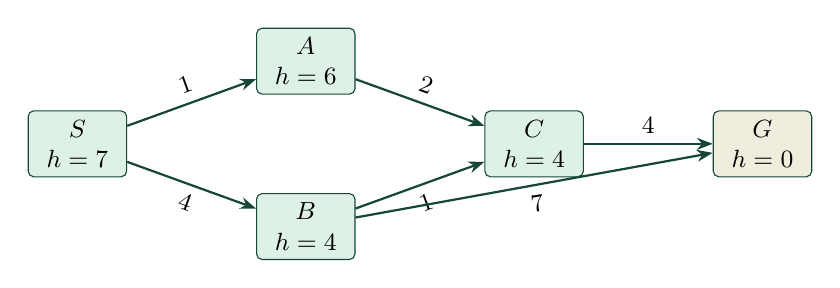
\begin{tikzpicture}[x=1.45cm,y=1.05cm]
      \node[reviewnode] (s) at (0,0) {$S$\\$h=7$};
      \node[reviewnode] (a) at (2,1) {$A$\\$h=6$};
      \node[reviewnode] (b) at (2,-1) {$B$\\$h=4$};
      \node[reviewnode] (c) at (4,0) {$C$\\$h=4$};
      \node[reviewgoal] (g) at (6,0) {$G$\\$h=0$};
      \draw[reviewarrow] (s) -- node[above,sloped,font=\small] {$1$} (a);
      \draw[reviewarrow] (s) -- node[below,sloped,font=\small] {$4$} (b);
      \draw[reviewarrow] (a) -- node[above,sloped,font=\small] {$2$} (c);
      \draw[reviewarrow] (b) -- node[below,sloped,font=\small] {$1$} (c);
      \draw[reviewarrow] (b) -- node[below,sloped,font=\small] {$7$} (g);
      \draw[reviewarrow] (c) -- node[above,sloped,font=\small] {$4$} (g);
    \end{tikzpicture}
  \end{center}
  Trace graph search from $S$. On every frontier entry, write $(g,h,f)$.
  \begin{activity}
    After expanding $S$, which node is expanded next: $A$ or $B$? Do not answer from the picture; compute $f$ for both.
  \end{activity}
\end{frame}

\begin{frame}{A$^*$ Solution: The Frontier Is the Whole Story}
  \small
  \begin{center}
    \renewcommand{\arraystretch}{1.4}
    \begin{tabular}{c|l|l}
      \textbf{Expand} & \textbf{New or improved frontier entries} & \textbf{Next choice} \\\hline
      $S$ & $A:(1,6,7)$, $B:(4,4,8)$ & $A$ \\
      $A$ & $C:(3,4,7)$, $B:(4,4,8)$ & $C$ \\
      $C$ & $G:(7,0,7)$, $B:(4,4,8)$ & $G$ \\
      $G$ & goal reached & stop
    \end{tabular}
  \end{center}
  The returned path is
  \[
    S\rightarrow A\rightarrow C\rightarrow G,
    \qquad \text{cost }7.
  \]
  \begin{keyidea}
    The heuristic did not make $B$ disappear; it only made $A$ and then $C$ more promising. A$^*$ still compares complete $f=g+h$ priorities, not intuition about which drawn route looks shorter.
  \end{keyidea}
\end{frame}

\section{Adversarial Search}

\begin{frame}{Minimax: Your Opponent Does Not Cooperate}
  In a deterministic, two-player, zero-sum game with perfect information:
  \begin{itemize}
    \item MAX chooses the child with the greatest backed-up value.
    \item MIN chooses the child with the smallest backed-up value.
    \item Leaf values are terminal utilities or heuristic estimates at a depth limit.
  \end{itemize}
  \[
    V_{\mathrm{MAX}}(s)=\max_{a\in Actions(s)}V(Result(s,a)),
    \qquad
    V_{\mathrm{MIN}}(s)=\min_{a\in Actions(s)}V(Result(s,a)).
  \]
  \begin{keyidea}
    Minimax does not predict the opponent's most likely action. It protects against their best action from their own point of view.
  \end{keyidea}
\end{frame}

\begin{frame}{Minimax Problem: Back Up the Leaves}
  \begin{center}
    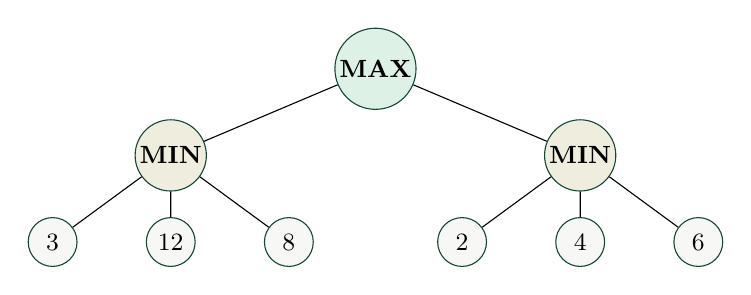
\begin{tikzpicture}[level distance=1.1cm,level 1/.style={sibling distance=5.2cm},level 2/.style={sibling distance=1.5cm}]
      \node[maxnode] {MAX}
        child {node[minnode] {MIN}
          child {node[leafnode] {$3$}}
          child {node[leafnode] {$12$}}
          child {node[leafnode] {$8$}}
        }
        child {node[minnode] {MIN}
          child {node[leafnode] {$2$}}
          child {node[leafnode] {$4$}}
          child {node[leafnode] {$6$}}
        };
    \end{tikzpicture}
  \end{center}
  \begin{activity}
    Work bottom-up. What does each MIN node return to the root? Which root action is selected? Explain why MAX cannot justify choosing the left child because one of its leaves is $12$.
  \end{activity}
\end{frame}

\begin{frame}{Minimax Solution: Every Player Optimizes Their Own Node}
  \begin{center}
    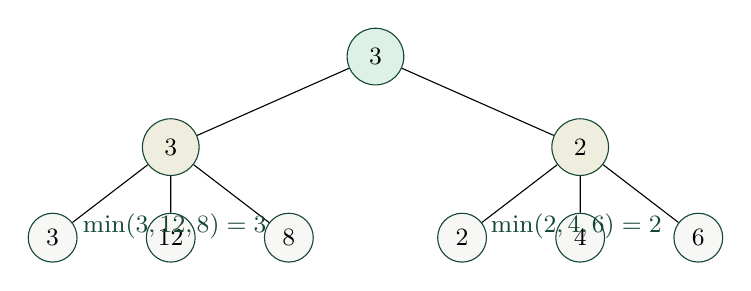
\begin{tikzpicture}[level distance=1.15cm,level 1/.style={sibling distance=5.2cm},level 2/.style={sibling distance=1.5cm}]
      \node[maxnode] {$3$}
        child {node[minnode] {$3$}
          child {node[leafnode] {$3$}}
          child {node[leafnode] {$12$}}
          child {node[leafnode] {$8$}}
        }
        child {node[minnode] {$2$}
          child {node[leafnode] {$2$}}
          child {node[leafnode] {$4$}}
          child {node[leafnode] {$6$}}
        };
      \node[font=\small,text=CalPolyGreen] at (-2.55,-2.15) {$\min(3,12,8)=3$};
      \node[font=\small,text=CalPolyGreen] at (2.55,-2.15) {$\min(2,4,6)=2$};
    \end{tikzpicture}
  \end{center}
  \[
    \max(3,2)=3.
  \]
  MAX chooses the \textbf{left} action. The $12$ is irrelevant because MIN, if given that subtree, chooses the $3$ instead.
  \begin{keyidea}
    Alpha-Beta pruning changes how many nodes we inspect, not the minimax value we eventually return.
  \end{keyidea}
\end{frame}

\section{First-Order Logic}

\begin{frame}{Forward Chaining: Make Every Rule Instance Whose Premises Are Known}
  \begin{itemize}
    \item A knowledge base contains facts and rules.
    \item \textbf{Forward chaining} begins with known facts and repeatedly applies rules whose premises match those facts.
    \item \textbf{Unification} finds a substitution that makes an abstract rule premise match a concrete fact.
    \item \textbf{Generalized modus ponens} adds the rule's instantiated conclusion.
  \end{itemize}
  \begin{keyidea}
    Forward chaining is data-driven: new facts trigger the rules that can use them. It is especially natural when you want every conclusion supported by the currently known data.
  \end{keyidea}
\end{frame}

\begin{frame}{Forward-Chaining Problem: What Can We Derive About Mina?}
  \small
  \begin{block}{Rules}
    \[
    \begin{aligned}
      \textit{Bird}(x) &\Rightarrow \textit{Animal}(x)\\
      \textit{Animal}(x)\land\textit{HasWings}(x) &\Rightarrow \textit{CanFly}(x)\\
      \textit{CanFly}(x)\land\textit{Healthy}(x) &\Rightarrow \textit{Cleared}(x)
    \end{aligned}
    \]
  \end{block}
  \begin{block}{Initial facts}
    \[
      \textit{Bird}(\textit{Mina}),\qquad
      \textit{HasWings}(\textit{Mina}),\qquad
      \textit{Healthy}(\textit{Mina}).
    \]
  \end{block}
  Apply forward chaining until no new fact can be produced. Record the substitution whenever a rule fires.
\end{frame}

\begin{frame}{Forward-Chaining Solution: New Facts Unlock Later Rules}
  \small
  \begin{enumerate}
    \item Match $\textit{Bird}(x)$ to $\textit{Bird}(\textit{Mina})$ with
    \[
      \{x/\textit{Mina}\}.
    \]
    Add $\textit{Animal}(\textit{Mina})$.
    \item Now $\textit{Animal}(\textit{Mina})$ and $\textit{HasWings}(\textit{Mina})$ satisfy the second rule with the same substitution. Add $\textit{CanFly}(\textit{Mina})$.
    \item Finally, $\textit{CanFly}(\textit{Mina})$ and $\textit{Healthy}(\textit{Mina})$ satisfy the third rule. Add $\textit{Cleared}(\textit{Mina})$.
  \end{enumerate}
  \begin{keyidea}
    The conclusion of one inference can become a premise for another. The process stops at a fixed point: no rule can add a fact that is not already known.
  \end{keyidea}
\end{frame}

\section{Bayesian Reasoning}

\begin{frame}{Naive Bayes: Compare Classes with Prior Times Likelihood}
  For class $C$ and observed features $x_1,\ldots,x_k$:
  \[
    P(C\mid x_1,\ldots,x_k)
    \propto P(C)\prod_i P(x_i\mid C).
  \]
  The proportionality sign means we may first compute unnormalized class scores and normalize only if a probability is required.
  \begin{keyidea}
    Naive Bayes assumes features are conditionally independent \emph{given the class}. The assumption is usually not literally true; the tradeoff is a compact model and cheap inference.
  \end{keyidea}
\end{frame}

\begin{frame}{Naive Bayes Problem: Classify an Email with Two Words}
  Let $S$ mean spam and $\neg S$ mean not spam.
  \[
  P(S)=0.40,\qquad P(\neg S)=0.60.
  \]
  \begin{center}
    \renewcommand{\arraystretch}{1.45}
    \begin{tabular}{c|cc}
      & $S$ & $\neg S$\\\hline
      $P(\textit{free}\mid\text{class})$ & $0.80$ & $0.10$\\
      $P(\textit{meeting}\mid\text{class})$ & $0.05$ & $0.60$
    \end{tabular}
  \end{center}
  An email contains both \textit{free} and \textit{meeting}.
  \begin{activity}
    Compute one score for spam and one for not spam. Then normalize to obtain $P(S\mid \textit{free},\textit{meeting})$.
  \end{activity}
\end{frame}

\begin{frame}{Naive Bayes Solution: The Words Pull in Opposite Directions}
  \small
  \[
    \text{score}(S)=0.40(0.80)(0.05)=0.016,
  \]
  \[
    \text{score}(\neg S)=0.60(0.10)(0.60)=0.036.
  \]
  Normalize with the total score $0.016+0.036=0.052$:
  \[
    P(S\mid \textit{free},\textit{meeting})
      =\frac{0.016}{0.052}\approx0.308.
  \]
  Therefore predict $\neg S$.
  \begin{keyidea}
    A feature can be strong evidence for spam without deciding the final label. Classification compares every class's prior-weighted explanation of \emph{all} observed features.
  \end{keyidea}
\end{frame}

\section{Bayesian-Network Sampling}

\begin{frame}{Prior Sampling: Generate Complete Worlds in Topological Order}
  In \textbf{prior sampling}, generate each Bayesian-network variable after its parents have been sampled.
  \begin{center}
    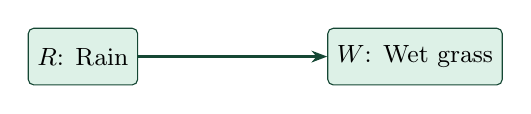
\begin{tikzpicture}[node distance=2.4cm]
      \node[reviewnode] (r) {$R$: Rain};
      \node[reviewnode,right=of r] (w) {$W$: Wet grass};
      \draw[reviewarrow] (r) -- (w);
    \end{tikzpicture}
  \end{center}
  Suppose
  \[
    P(R)=0.30,\qquad P(W\mid R)=0.90,\qquad P(W\mid\neg R)=0.10.
  \]
  \begin{keyidea}
    A prior sample is a synthetic complete assignment drawn from the model's joint distribution. Estimate a probability by the fraction of generated worlds in which the event occurs.
  \end{keyidea}
\end{frame}

\begin{frame}{Prior-Sampling Problem: Estimate $P(W)$ from Samples}
  A sampling run produces these ten complete assignments:
  \begin{center}
    \renewcommand{\arraystretch}{1.35}
    \begin{tabular}{c|cccccccccc}
      sample & 1 & 2 & 3 & 4 & 5 & 6 & 7 & 8 & 9 & 10\\\hline
      $R$ & T & F & F & T & F & F & F & T & F & F\\
      $W$ & T & F & F & T & F & F & F & F & T & F
    \end{tabular}
  \end{center}
  \begin{activity}
    Estimate $P(W)$ from this run. Then explain why the estimate is not required to equal the exact answer, even though every sample was generated correctly.
  \end{activity}
\end{frame}

\begin{frame}{Prior-Sampling Solution: Count Worlds, Then Remember the Error Bar}
  Wet grass appears in samples $1$, $4$, and $9$:
  \[
    \widehat{P}(W)=\frac{3}{10}=0.30.
  \]
  The exact value from enumeration would be
  \[
    P(W)=P(R)P(W\mid R)+P(\neg R)P(W\mid\neg R)
         =0.30(0.90)+0.70(0.10)=0.34.
  \]
  \begin{keyidea}
    Sampling trades exactness for scalability. With more independent samples, the estimate should converge toward the model's probability, but any finite run can be high or low by chance.
  \end{keyidea}
\end{frame}

\section{Kalman Filtering}

\begin{frame}{A One-Dimensional Kalman Filter Alternates Predict and Correct}
  We represent belief about position as a Gaussian:
  \[
    x\sim\mathcal{N}(\mu,P).
  \]
  \begin{itemize}
    \item $\mu$ is the estimated position.
    \item $P$ is uncertainty, represented here as variance.
    \item Motion changes the expected position and adds process uncertainty $Q$.
    \item A sensor reports $z$ with measurement variance $R$.
  \end{itemize}
  For our simple position model:
  \[
    \bar\mu=\mu+u,\qquad \bar P=P+Q,
  \]
  \[
    K=\frac{\bar P}{\bar P+R},\qquad
    \mu'=\bar\mu+K(z-\bar\mu),\qquad
    P'=(1-K)\bar P.
  \]
  \begin{keyidea}
    The Kalman gain $K$ determines how strongly the update trusts the measurement relative to the predicted belief.
  \end{keyidea}
\end{frame}

\begin{frame}{Kalman Problem: Move, Then Read One Noisy Sensor}
  A robot begins with
  \[
    x_0\sim\mathcal{N}(10,1).
  \]
  It commands a move of $u=5$. Motion has variance $Q=4$.
  After moving, a position sensor reports $z=17$ with variance $R=4$.
  \begin{enumerate}
    \item Predict the belief after motion: compute $\bar\mu$ and $\bar P$.
    \item Compute the Kalman gain $K$.
    \item Update the mean $\mu'$ and variance $P'$ after seeing the sensor reading.
  \end{enumerate}
  \begin{activity}
    Before calculating: should the posterior mean land at $15$, at $17$, or strictly between them? Why?
  \end{activity}
\end{frame}

\begin{frame}{Kalman Solution, Step 1: Prediction Follows the Motion Model}
  The commanded move shifts the estimated position by five units:
  \[
    \bar\mu=10+5=15.
  \]
  Motion noise increases uncertainty:
  \[
    \bar P=1+4=5.
  \]
  Before reading the sensor, the belief is
  \[
    x\sim\mathcal{N}(15,5).
  \]
  \begin{keyidea}
    A prediction is not merely ``add the movement.'' It must also acknowledge that real motion is imperfect, so uncertainty grows before the measurement arrives.
  \end{keyidea}
\end{frame}

\begin{frame}{Kalman Solution, Step 2: Correct Toward the Measurement}
  \small
  The gain is
  \[
    K=\frac{5}{5+4}=\frac{5}{9}\approx0.556.
  \]
  The sensor is two units above the prediction, so move $55.6\%$ of that gap:
  \[
    \mu'=15+\frac{5}{9}(17-15)
         =15+\frac{10}{9}
         \approx16.11.
  \]
  The corrected variance is
  \[
    P'=(1-\tfrac{5}{9})(5)=\frac{20}{9}\approx2.22.
  \]
  \begin{keyidea}
    The posterior lies between prediction and measurement, and it is more certain than either alone. Equal-sized predicted and measurement variances would have produced $K=0.5$.
  \end{keyidea}
\end{frame}

\section{Markov Decision Processes}

\begin{frame}{MDPs: Choose for the Future, Not Just the Immediate Reward}
  A Markov Decision Process is commonly written
  \[
    \langle S,A,T,R,\gamma\rangle.
  \]
  \begin{itemize}
    \item $S$: states; $A$: actions available in each state.
    \item $T(s,a,s')$: transition probability to next state $s'$.
    \item $R(s,a,s')$: immediate reward for that transition.
    \item $\gamma$: discount factor; a \textbf{policy} chooses an action in each state.
  \end{itemize}
  A one-step action-value backup is
  \[
    Q(s,a)=\sum_{s'}T(s,a,s')\left[R(s,a,s')+\gamma V(s')\right].
  \]
  \begin{keyidea}
    MDP planning assumes the transition and reward model are known. Reinforcement learning instead estimates useful values from experience.
  \end{keyidea}
\end{frame}

\begin{frame}{Small MDP Problem: Deliver Now or Recharge First?}
  At state \textit{Low battery}, use $\gamma=0.9$. Suppose later planning has supplied
  \[
    V(\textit{Charged})=10,\qquad V(\textit{Delivered})=0,\qquad V(\textit{Stalled})=-5.
  \]
  \begin{center}
    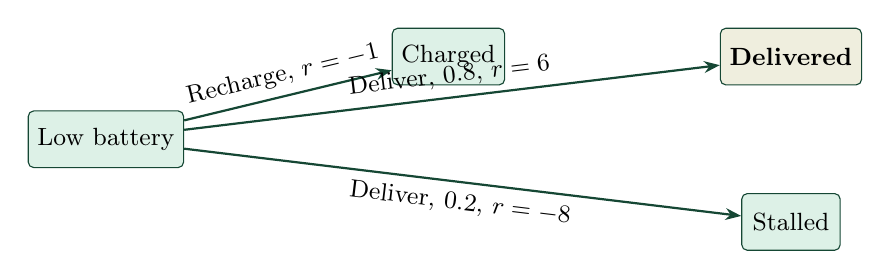
\begin{tikzpicture}[x=1.45cm,y=1.05cm]
      \node[reviewnode] (low) at (0,0) {Low battery};
      \node[reviewnode] (charge) at (3,1) {Charged};
      \node[reviewgoal] (del) at (6,1) {Delivered};
      \node[reviewnode] (stall) at (6,-1) {Stalled};
      \draw[reviewarrow] (low) -- node[above,sloped,font=\small] {Recharge, $r=-1$} (charge);
      \draw[reviewarrow] (low) -- node[above,sloped,font=\small] {Deliver, $0.8$, $r=6$} (del);
      \draw[reviewarrow] (low) -- node[below,sloped,font=\small] {Deliver, $0.2$, $r=-8$} (stall);
    \end{tikzpicture}
  \end{center}
  Compute $Q(\textit{Low},\textit{Recharge})$ and $Q(\textit{Low},\textit{Deliver})$.
\end{frame}

\begin{frame}{Small MDP Solution: Delayed Value Can Beat Immediate Progress}
  \small
  Recharge has one possible transition:
  \[
    Q(\textit{Low},\textit{Recharge})=-1+0.9(10)=8.
  \]
  Deliver has two possible transitions:
  \[
  \begin{aligned}
    Q(\textit{Low},\textit{Deliver})
      &=0.8\left[6+0.9(0)\right]
        +0.2\left[-8+0.9(-5)\right]\\
      &=4.8-2.5=2.3.
  \end{aligned}
  \]
  The policy should choose \textbf{Recharge}, even though it has immediate reward $-1$.
  \begin{keyidea}
    Greedy action selection sees $6>-1$ and delivers immediately. MDP reasoning includes the next state's value and the risk of reaching a bad future state.
  \end{keyidea}
\end{frame}

\begin{frame}{Exam Checklist: What Should You Write Before You Calculate?}
  \small
  \begin{enumerate}
    \item \textbf{Search:} frontier entries and the priority rule ($g$, $h$, $f$).
    \item \textbf{Games:} whose node it is and whether to take max, min, or an expectation.
    \item \textbf{Logic:} facts, rule premises, and substitutions that make them match.
    \item \textbf{Bayes:} prior, likelihood, competing hypotheses, then the normalizing denominator.
    \item \textbf{Sampling:} what each sample represents and what fraction or weighted fraction estimates the query.
    \item \textbf{Filtering:} predicted mean/variance before the sensor, then gain and corrected belief.
    \item \textbf{MDPs:} next states, their probabilities, immediate rewards, discount, and future values.
  \end{enumerate}
  \begin{keyidea}
    Most lost points come from silently switching representations: treating a likelihood as a posterior, a heuristic as true cost, a reward as a return, or a leaf value as a policy value.
  \end{keyidea}
\end{frame}

\begin{frame}{Closing: Seven Problems, One Habit}
  Every technique today uses a representation to make a difficult reasoning problem tractable.
  \begin{center}
    \renewcommand{\arraystretch}{1.45}
    \begin{tabular}{l|l}
      A$^*$ & cost-so-far plus admissible estimate \\
      Minimax & alternating optimal choices \\
      Forward chaining & facts and rule instances \\
      Naive Bayes & prior-weighted, conditionally independent evidence \\
      Prior sampling & complete worlds drawn from a model \\
      Kalman filtering & Gaussian belief updated by noisy motion and sensing \\
      MDPs & stochastic actions plus long-run value
    \end{tabular}
  \end{center}
  \begin{keyidea}
    On the midterm, name the representation first. Then carry the semantics of each number all the way through the calculation.
  \end{keyidea}
\end{frame}

\end{document}